\chapter{Social network visualization}

Even though the data mining processes described in the previous chapters give us valuable insights into the structure of social networks, 
they are not necessarily easy to interpret for laymen.
One way to make the results of data mining more accessible is to create data visualization, i.e. present the data with their visual representation, 
while using different visual cues to guide the viewers' attention towards different qualities.

In this part of the thesis, we will assess the current state of the visualizations in the Charles Explorer application, 
will propose some improvements to make the visualization more accessible to the users and will implement those.

\section{Vocabulary}

This section introduces some basic vocabulary that will be used throughout this chapter.

\textbf{Ego network}: Ego-centric networks (or shortened to “ego” networks) are a particular type of network which specifically maps the connections of and from the perspective of a single person (an “ego”). (\cite{Lizardo2020-xo}).

\textbf{Visual decoding}: Also called \textit{preattentive processing} or \textit{preattentive vision}, the visual decoding is the instantaneous perception of the visual field that comes without apparent mental effort. (\cite{Cleveland1985})

\section{Assessing the current state}

The current state of the Charles Explorer visualization views is quite simple. 

In the \textit{Person} search mode, the user can search for people inside the Charles University. 
When accessing a person's profile, the application shows the person's \textit{ego network} with the main person and their direct collaborators 
as nodes and their common publications aggregated to the edges.

\begin{figure}[ht!]
    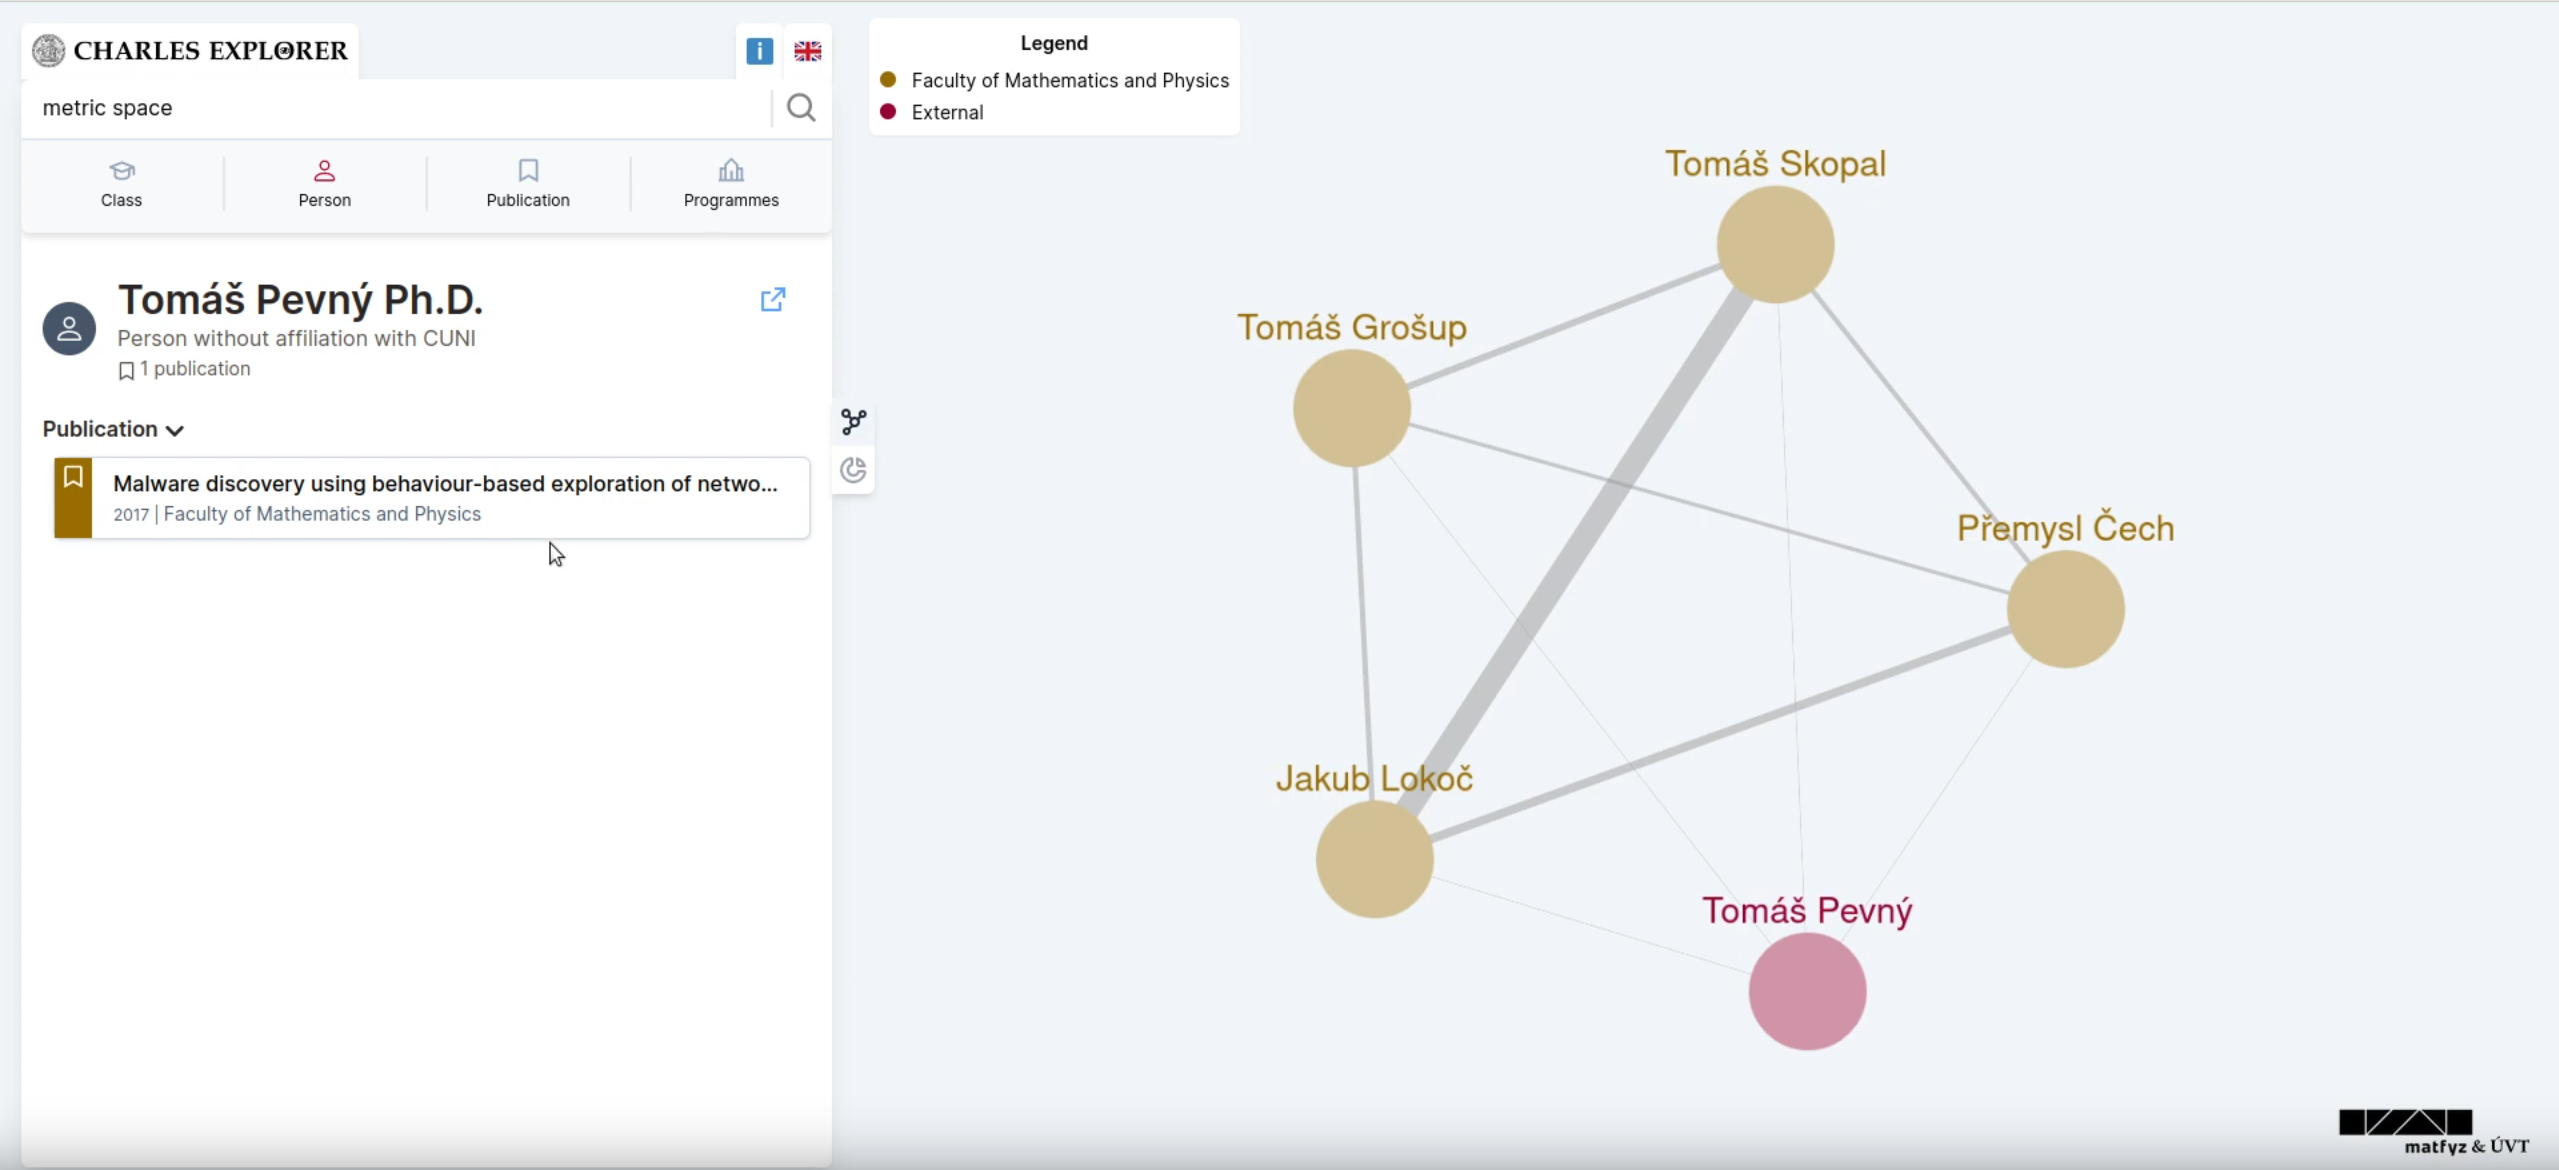
\includegraphics[width=0.8\textwidth]{../img/charles-explorer-old-view.png}
    \centering
    \caption{Charles Explorer showing the \textit{ego network} of a person.}
\end{figure}

The graph is displayed with force-directed layout. The edge thickness is proportional to the number of common publications between 
the two people and the colors of the nodes represent the person's faculty association.

This approach has multiple drawbacks which we will now address and discuss.

\subsection{Problems with color coding}

Firstly, the color coding of the nodes does not prove very useful, as it hinders the \textit{visual decoding} of the graph.
The user spends more attention on reading the legend, rather than interpreting the graph subconciously.

This is especially true for larger ego networks with many nodes with different faculty affiliations. 
Additionaly, the application does not provide any alternative visual cue for color vision deficient users.

According to \cite{Cleveland1985}, the discriminability of colors by people is limited to 5 - 6 colors. This is not enough for the 17 faculties and departments 
of the Charles University. With faculties, there is also little room for a meaningful aggregation (of multiple faculties into one color), as the faculty structure is not 
hierarchical.

\subsection{Layouting problems}

The arbitrary positions of the nodes based on the physical simulation layout increase the cognitive load 
of the viewer and contribute to the graph's worse readability.

\cite{munzner2015visualization} states that the position of data points on a common scale is the most effective way to communicate the data to the viewer.
By using the physical simulation layout, we are willingly giving up this visual channel (the x and y position of the nodes in the screen space).


\subsection{Other visualization problems}

\section{Graph layouting algorithms}

Before we start, let us introduce some basic terminology that will be used throughout this chapter.

A \emph{graph layout} is a way to position the nodes of a graph in a two-dimensional space, such as on a screen or in print. 
This is a necessary step of any graph data visualisation task - without computing the layout, the graph nodes nor edges do not have any intrinsic location assigned to them.

There are several various ways of computing the graph layout, which we'll describe now in no particular order:

\begin{itemize}
    \item \textbf{Hierarchical layout} - for certain types of graphs, it's beneficial to display them in a hierarchical manner. 
    This is usually the case for trees, i.e. connected acyclic graphs - such as family trees or organisation structures.

    Such layout is typically laid out on either horizontal or vertical axis, with the root node at the top or leftmost position, and the children nodes below or to the right of their parent nodes.
    The other direction (i.e. vertical for horizontal-major graphs and vice versa) is used for layouting the incomparable sibling groups.
    
    While this layout might be used on cyclic graphs as well, it's not as common, as it's not as easy to interpret for laymen as the other layouts.
    It might be useful for graphs with some kind of hierarchy or other clear ``score'' quality, such as social networks with a clear leader, or a company structure.

    \item \textbf{Circular layout} - this layout places the nodes on a circle, with the edges connecting them. 
    This layout is useful for visualizing relations between members of a group or community, as it's easy to see which nodes are connected to which other nodes.
    Some work can be done for calculating the optimal placement of nodes - be it minimizing the edge length, or minimizing the number of edge crossings.

    While minimizing the number of edge crossings might help with the graph readability, it might result in a less visually appealing graph, as the nodes might be placed further apart than necessary.
    % TODO: add a reference to the paper about this.

    Trying to minimize the edge length by ordering the nodes on the circle also results in a more readable graph, as this layout promotes grouping closely connected subcommunities together.

    In some cases, the global position of nodes in the layout can depict some qualitative variable - e.g. in a social network of people from different social groups, 
    the node position on the y-axis might represent the person's annual income. With the edges between the nodes representing the social connections,
    such layout can help us understand the relation between the social status and the connections between the people.

    \item \textbf{Grid layout} - this layout places the nodes on a grid, with the edges connecting them.
    While some optimizations, such as minimizing the edge length can be done in this case as well, 
    this type of layout usually results in a less readable graph.

    An equally-spaced grid layout only communicates the relations between nodes by drawing the edges between them, not utilising the position of the nodes.
    It is often the spatial proximity of the nodes that helps viewers understand the relations between the nodes subconciously - and while we still can 
    supply this information by using different visual cues (e.g. coloring of the nodes), it's often not as intuitive as the spatial proximity.

    Unlike the hierarchical and circular layouts, there does not seem to be a clear use for the global node position for depicting some qualitative variable.

    In some applications, the grid layout is sometimes used as the initial graph layout for the force-directed layout, as it's easier to calculate the initial positions of the nodes on a grid.

    \item \textbf{Force-directed layout} - this layout is based on the physical simulation of the forces between the nodes and edges of the graph.
    The nodes are treated as charged particles, and the edges as springs - the nodes repel each other, while the edges try to keep the nodes connected.
    
    This results in a layout where the nodes are placed in such a way that the edges are as short as possible, while the nodes are as far apart as possible.
    This is useful for visualizing the overall structure of the graph, as it's easy to see which nodes are connected to which other nodes, and how the graph is connected.

    Using the edges to guide the layouting process results in a more ``intuitively'' readable graph, as the edges representing some sort of relation between two nodes 
    cause the nodes to be drawn to each other. This means that related nodes are layouted closer to each other - therefore supporting the spatial proximity Gestalt principle.

    The force-directed layout is especially useful for visualizing large social networks, as it's easy to see which nodes are connected to which other nodes, and how the graph is connected.
    Such graph is also easy to navigate, and the viewer can easily find bridges, hubs, or other important features of the graph.

    Similar to the grid layout, the global node position cannot be used to depict qualitative variables. While it might be technically possible 
    to add auxiliary forces to the simulation to achieve this - e.g. pull nodes to the left or right of the screen based on some variable - 
    it's not as common as in the hierarchical or circular layouts. This approach might also interfere with the edge-based layouting process,
    causing the graph to be less readable.

    Because of this reason and the very essence of the force-directed layouts, the location of the nodes in such layout is quite arbitrary 
    - in case of large graphs, the viewer might not be able to find the node they are looking for. This is why it's often useful to add 
    some sort of search functionality or other navigation aids to the visualization.
\end{itemize}
